% !TEX root = stack-thresh.tex


%%%%%%%%%%%%%%%%%%%%%%%%%%%%%%%%%%%%%%%%%%%%%%%%%%%%%%%%%%%%%%%%%%%%%%%%%%%%%%%%
\section{The cost of Stackelberg equilirbia}
\label{sec:cost}

As in the previous section, we consider Stackelberg instances with a fixed number of links, fixed demand, and variable compliance rate. We derive the analytical expression of the optimal Stackelberg cost,  which we will denote by $C_{\textup{NCF}}(\cR)$, as a function of the compliance rate $\compRate \in [0,1[$\footnote{We exclude the case where the coordinator has total control ($\compRate = 1$) to simplify the discussion: in this case the non-compliant flow is zero and the last link in its support, $\lastNC{1}$ is not defined. The analysis in this case needs a slightly different notation.}. Since the NCF strategy~$\sV^{(\cR)}$ is an optimal Stackelberg strategy, the optimal Stackelberg cost is simply given by
\begin{align}
C_{\textup{NCF}}(\cR) 
&= C(\sV^{(\cR)} + \tV^{(\cR)}, \modeV^{(\cR)})\\
&= C(\flowV^{(\cR)}, \modeV^{(\cR)})\\
&= \sum_{n=1}^{\lastStack{\cR}} \flow^{(\cR)} \latency_n(\flow^{(\cR)}, \mode^{(\cR)}) \label{eq:stackCost}
\end{align}
The main result is that $C_{\textup{NCF}}(\cR)$ is a non-increasing, piecewise-constant function of $\cR$ with discontinuities exactly at the points $\left\{1- \frac{ \maxR{j} }{ \demand } \right\}_{1 \leq j < j_0}$ where $k_j$ are the links that strictly increase the maximum demand, as defined in Section~\ref{sec:previous-Nash}, and $j_0$ is such that the last link in the support of the best Nash equilibrium $\std \BNE$ is $\lastNC{0} = k_{j_0}$.\\

We define intervals $I_1, \dots, I_{j_0}$ as follows:
\begin{itemize}
\item $I_1 = \left[1- \frac{\maxR{1}}{\demand}, 1\right[ = \left[1- \frac{\demandMax{1}}{\demand}, 1\right[$
\item For $1 < j \leq j_0$, ${ I_j = \left[ 1- \frac{\maxR{j}}{\demand}, 1- \frac{\maxR{j-1}}{\demand} \right[ }$
\end{itemize}

\begin{proposition}
\label{prop:j_0}
The interval $I_{j_0}$ satisfies $0 \in I_{j_0}$.
\end{proposition}

\begin{proof}
By~\eqref{eq:lastNC2}, we have
\[
k_{j_0} = \lastNC{0} = \min \{k : \demand \leq \demandMax{k}\}
\]
thus $\demand \leq \demandMax{k_{j_0}}$ and $\demand > \demandMax{k_{j_0 - 1}}$, i.e.
$1 - \frac{\demandMax{k_{j_0}}}{\demand} \leq 0$ and $1 - \frac{\demandMax{k_{j_0 - 1}}}{\demand} > 0$.

\end{proof}

Note that the intervals are disjoint by definition, and by Proposition~\ref{prop:j_0}, ${ [0, 1] \subset I_{j_0} \cup \dots \cup I_1 }$. See Fig.~\ref{fig:intervals} for an illustration of the intervals $\{ I_j \}_{1 \leq j \leq j_0}$.

\begin{figure}[h]
\centering
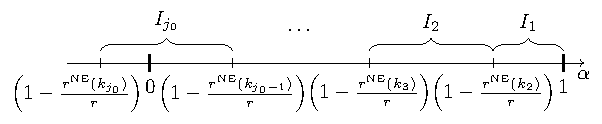
\includegraphics[width=3.4in]{TikZ/intervals.pdf}
\caption{Intervals $\{ I_j \}_{1 \leq j \leq j_0}$.}
\label{fig:intervals}
\end{figure}

First, we prove that on each interval $I_j$, the optimal Stackelberg cost is constant. 

From the expression~\eqref{eq:NCF-totalFlow} of the total flow $\flowV^{(\cR)}$ and the expression~\eqref{eq:NCF-ncMode} of the congestion states, the optimal Stackelberg cost is given by
\begin{multline}
C_{\textup{NCF}}(\compRate) = 
\bigg( \sum_{n = 1}^{\lastNC{\compRate} - 1} \cFlow{n}{\lastNC{\compRate}} \bigg) a_{\lastNC{\compRate}} + \\
\bigg( \sum_{n = \lastNC{\compRate}}^{\lastStack{\compRate} - 1} \flowMax_n a_n\bigg) + 
\flow^{(\cR)}_{\lastStack{\compRate}} a_{\lastStack{\compRate}}
\label{eq:cost}
\end{multline}

In this expression, several terms appear to depend on $\cR$: $\lastNC{\cR}$, $\lastStack{\cR}$ and $\flow^{(\cR)}_{\lastStack{\cR}}$. However, we show that when $\compRate \in I_j$, these terms are constant.
%


\begin{lemma}
\label{lem:cost}
Let $j \in \{1, \dots, j_0 \}$. Then $\forall \compRate \in I_j$, $\lastNC{\cR}$ is constant and equal to $k_j$, $\lastStack{\cR}$ is constant, and the optimal Stackelberg cost $C_{\textup{NCF}}(\cR)$ is constant.
\end{lemma}

\begin{proof}
Let $j \in \{1, \dots, j_0\}$ and let $\compRate \in I_j$. We first show that $\lastNC{\cR} = k_j$. 

For $j \in \{1, \dots, j_0\}$, we have by definition of $I_j$
\[
\compRate \in I_j \Leftrightarrow \demandMax{k_{j-1}} < (1-\compRate)\demand \leq  \demandMax{k_j}
\]
(by convention, we let $k_0 = 0$ and $\demandMax{0} = 0$ so that this statement is true for $j=1$). By the inductive definition~\eqref{eq:nj} of $k_j$, we have $\forall n < k_j$, $\demandMax{n} \leq \demandMax{k_{j-1}}$, thus $\forall n < k_j$, $\demandMax{n} < (1-\compRate)\demand$. Therefore $k_j$ is the minimal index such that $(1-\compRate)\demand \leq \demandMax{k_j}$, i.e. $k_j = \lastNC{\compRate}$ by characterization~\eqref{eq:lastNC}.


Next, since $\lastNC{\compRate}$ is constant, so are $\lastStack{\compRate}$ and $\flowV^{(\cR)}$ by Proposition~\ref{prop:lastStack_constant}. Finally, from~\eqref{eq:cost} the optimal Stackelberg cost is constant since all terms are constant.
\end{proof}

For $\compRate \in I_j$, we will denote by $l_j$ the constant value of $\lastStack{\cR}$, and by $C_j$ the constant value of $C_{\textup{NCF}}(\compRate)$. Note that $l_j$ is by definition
\begin{equation}
\label{eq:l_j}
l_j = \max \bigg\{ l : \demand - \bigg( \maxR{j} + \sum_{n=k_j+1}^{l-1}{\flowMax_n} \bigg) > 0 \bigg\}
\end{equation}


As a consequence of the previous Lemma, the optimal Stackelberg cost is piecewise constant as a function of the compliance rate $\cR$. The next theorem shows that it is a non-increasing function and specifies points of discontinuity.

\begin{theorem}{\emph{Optimal Stackelberg cost}\\}
\label{thm:cost}
The optimal Stackelberg cost $C_{\textup{NCF}}(\alpha)$ is a non-increasing, piecewise-constant function of $\cR \in [0,1[$ with discontinuities exactly at the points $\left\{ 1- \frac{\maxR{j}}{\demand} \right\}_{1 \leq j < j_0}$. On each $I_j$, ${ 1 \leq j \leq j_0 }$, its constant value $C_j$ is given by
\begin{multline}
C_j = 
\bigg( \sum_{n = 1}^{k_j - 1} \cFlow{n}{k_j} \bigg) a_{k_j} + 
\bigg( \sum_{n = k_j}^{l_j - 1} \flowMax_n  a_n \bigg)+ \\
\bigg[\demand - \sum_{n = 1}^{k_j - 1} \cFlow{n}{k_j} - \sum_{n = k_j}^{l_j-1}{\flowMax_n} \bigg] a_{l_j}
\end{multline}
where $l_j$ is given by \eqref{eq:l_j}.
\end{theorem}
\begin{proof}
We need to prove that if $j > i$, then $C_j > C_i$. Let $i, j \in \{1, \dots, j_0 - 1\}$, such that $j > i$ and let $\compRate_i \in I_i$ and $\compRate_j \in I_j$.

We have by Lemma~\ref{lem:cost}, $\lastNC{\cR_i} = k_i$ and $\lastNC{\cR_j} = k_j$. We also have
\begin{itemize}
\item $k_i<k_j$ (since $i<j$)
\item $l_i \leq l_j$ (we have by definition of $I_i$ and $I_j$, $\compRate_i > \compRate_j$, thus by Lemma~\ref{lem:lastStack_decreasing}, $\lastStack{\cR_i} \leq \lastStack{\cR_j}$)
\item $l_i > k_i$ (we have by definition $l_i \geq k_i$. If we have equality, then we have a single-link-free-flow equilibrium supported on $\{1, \dots, k_i\}$, thus $\demand \leq \maxR{i}$, but $k_i < k_j \leq k_{j_0} = \min \{ k | \demand \leq \demandMax{k} \} $, contradiction).
\end{itemize}

We now use the expression~\eqref{eq:NCF-totalFlow} to compare the flows $\flowV^{(\cR_i)}$ and~$\flowV^{(\cR_j)}$.

First, we have $\forall n \in \{1, \dots, k_i-1\}$, $\flow_n^{(\cR_i)} = \cFlow{n}{k_i}$ and $\flow_n^{(\cR_j)} = \cFlow{n}{k_j}$ and since $k_i < k_j$, we have $\cFlow{n}{k_i} > \cFlow{n}{k_j}$ ($\cFlow{n}{\cdot}$ is decreasing). The latencies are given by $\latency_n(\flow_n^{(\cR_j)}, \mode_n^{(\cR_j)}) = a_{k_j}$ and $\latency_n(\flow_n^{(\cR_i)}, \mode_n^{(\cR_i)}) = a_{k_i}$. Thus
\begin{multline}
\forall n \in \{1, \dots, k_i - 1\},
\flow_n^{(\cR_i)} > \flow_n^{(\cR_j)} > 0 \text{ and } \\ 
\latency_n(\flow_n^{(\cR_j)}, \mode_n^{(\cR_j)}) > \latency_n(\flow_n^{(\cR_i)}, \mode_n^{(\cR_i)})
\label{eq:thm_proof_1}
\end{multline}

Second, we have for $n = k_i$, $\flow_{k_i}^{(\cR_i)} = \flowMax_{k_i} $ (since $l_i > k_i$) and $\flow_{k_i}^{(\cR_j)} = \cFlow{n}{k_j}$ (since $k_i < k_j$). Therefore
\begin{equation}
\flow_{k_i}^{(\cR_i)} > \flow_{k_i}^{(\cR_j)} > 0  
\label{eq:thm_proof_2}
\end{equation}

Third, we have $\forall n \in \{k_i, \dots, l_i-1\}$, $\flow_n^{(\cR_i)} = \flowMax_n$, and $\latency_n(\flow_n^{(\cR_i)}, \mode_n^{(\cR_i)}) = a_n$. By definition of the maximum flow, we have $\flow_n^{(\cR_j)} \leq \flowMax_n$, and by definition of the free-flow latency $a_n$, $\latency_n(\flow_n^{(\cR_j)}, \mode_n^{(\cR_j)}) \geq a_n$. Thus
\begin{multline}
\forall n \in \{k_i, \dots, l_i - 1\}, \flow_n^{(\cR_i)} \geq \flow_n^{(\cR_j)} \text{ and } \\
\latency_n(\flow_n^{(\cR_j)}, \mode_n^{(\cR_j)}) \geq \latency_n(\flow_n^{(\cR_i)}, \mode_n^{(\cR_i)})
\label{eq:thm_proof_3}
\end{multline}

Finally, we have $\forall n \in \{l_i, \dots, l_j\}$, $\latency_n(\flow_n^{(\cR_j)}, \mode_n^{(\cR_j)}) \geq a_n$ by definition of the latency function, and $a_n \geq a_{l_i}$ (by the ordering of the links). Thus
\begin{equation}
\forall n \in \{l_i, \dots, l_j\}, \latency_n(\flow_n^{(\cR_j)}, \mode_n^{(\cR_j)}) \geq a_{l_i}
\label{eq:thm_proof_4}
\end{equation}

Using the expression~\eqref{eq:stackCost} of the optimal Stackelberg cost, we have
\begin{align}
C_j 
&= \sum_{n = 1}^{l_j} \flow_n^{(\cR_j)} \latency_n(\flow_n^{(\cR_j)}, \mode_n^{(\cR_j)}) \notag \\
&= \sum_{n = 1}^{l_i-1} \flow_n^{(\cR_j)} \latency_n(\flow_n^{(\cR_j)}, \mode_n^{(\cR_j)}) + 
\sum_{n = l_i}^{l_j} \flow_n^{(\cR_j)} \latency_n(\flow_n^{(\cR_j)}, \mode_n^{(\cR_j)}) \notag \\
&\geq \sum_{n = 1}^{l_i-1} \flow_n^{(\cR_j)} \latency_n(\flow_n^{(\cR_j)}, \mode_n^{(\cR_j)}) + 
\bigg(\sum_{n = l_i}^{l_j} \flow_n^{(\cR_j)} \bigg) a_{l_i} \label{eq:thm_proof_5}\\
&> \sum_{n = 1}^{l_i-1} \flow_n^{(\cR_j)} \latency_n(\flow_n^{(\cR_i)}, \mode_n^{(\cR_i)}) + 
\bigg(\sum_{n = l_i}^{l_j} \flow_n^{(\cR_j)} \bigg) a_{l_i} \label{eq:thm_proof_6}
\end{align}
where inequality~\eqref{eq:thm_proof_5} follows from~\eqref{eq:thm_proof_4}, and inequality~\eqref{eq:thm_proof_6} follows from the fact that ${ \forall n \in \{1, \dots, l_i - 1\} }$,  ${ \flow_n^{(\cR_j)}\latency_n(\flow_n^{(\cR_j)}, \mode_n^{(\cR_j)}) \geq \flow_n^{(\cR_j)}\latency_n(\flow_n^{(\cR_i)}, \mode_n^{(\cR_i)}) }$, with strict inequality for $n \leq k_i$ by~\eqref{eq:thm_proof_1},~\eqref{eq:thm_proof_2} and~\eqref{eq:thm_proof_3}.

We then use the fact that $l_j$ is the last link in the support of $\flowV^{(\cR_j)}$, thus $\demand = \sum_{n = 1}^{l_j} \flow_n^{(\cR_j)}$, i.e.
\[
\sum_{n = l_i}^{l_j} \flow_n^{(\cR_j)} = \demand - \sum_{n = 1}^{l_i - 1} \flow_n^{(\cR_j)}
\]
plugging this in the previous inequality, we have
\begin{align*}
C_j 
&> \bigg( \sum_{n = 1}^{l_i-1} \flow_n^{(\cR_j)} \big( \latency_n(\flow_n^{(\cR_i)}, \mode_n^{(\cR_i)}) - a_{l_i} \big) \bigg)+ \demand a_{l_i}
\end{align*}
We have $\forall n \in \{1, \dots, l_i - 1\}$, $\latency_n(\flow_n^{(\cR_i)}, \mode_n^{(\cR_i)}) - a_{l_i} \leq 0$, and $\flow_n^{(\cR_j)} - \flow_n^{(\cR_i)} \leq 0$, thus
\[
\flow_n^{(\cR_j)} \big( \latency_n(\flow_n^{(\cR_i)}, \mode_n^{(\cR_i)}) - a_{l_i} \big) \geq 
\flow_n^{(\cR_i)} \big( \latency_n(\flow_n^{(\cR_i)}, \mode_n^{(\cR_i)}) - a_{l_i} \big)
\]
plugging this in the previous inequality and rearranging the terms, we obtain
\begin{align*}
C_j 
&> \bigg( \sum_{n = 1}^{l_i-1} \flow_n^{(\cR_i)} \big( \latency_n(\flow_n^{(\cR_i)}, \mode_n^{(\cR_i)}) - a_{l_i} \big) \bigg)+ \demand a_{l_i} \\
&= \bigg( \sum_{n = 1}^{l_i-1} \flow_n^{(\cR_i)} \latency_n(\flow_n^{(\cR_i)}, \mode_n^{(\cR_i)}) \bigg)+ \bigg( \demand - \sum_{n = 1}^{l_i-1} \flow_n^{(\cR_i)} \bigg) a_{l_i} \\
&= C_i
\end{align*}
which competes the proof.
\end{proof}